\documentclass[10pt,twocolumn,letterpaper]{article}

\usepackage[review]{cvpr}

% Additional packages not loaded by cvpr.sty
\usepackage{multirow}
\usepackage{algorithm}
\usepackage{algorithmic}

\definecolor{cvprblue}{rgb}{0.21,0.49,0.74}
\usepackage[pagebackref,breaklinks,colorlinks,allcolors=cvprblue]{hyperref}

\definecolor{budgetgreen}{RGB}{0,158,115}
\definecolor{fixedblue}{RGB}{0,114,178}
\definecolor{growred}{RGB}{213,94,0}

\def\paperID{*****}
\def\confName{CVPR}
\def\confYear{2026}

\graphicspath{{../figures/}}

\title{BudgetNAS: Continual Online Neural Architecture Search\\with Budgeted Architecture Mutation}

\author{
Anonymous CVPR-NAS26 Submission
}

\begin{document}
\maketitle

% ============================================================
% ABSTRACT
% ============================================================
\begin{abstract}
Deploying deep learning models in non-stationary environments requires architectures that can adapt to distribution shifts. Existing NAS methods assume fixed data distributions, while continual learning methods operate on fixed architectures. We propose \textbf{BudgetNAS}, a framework for \emph{continual online NAS} that mutates a deployed model's architecture under a strict per-domain mutation budget~$B$. We evaluate ten methods---spanning fixed-architecture baselines, naive growth strategies, continual learning methods, and three BudgetNAS variants---on a three-domain streaming benchmark (CIFAR-10 $\rightarrow$ CIFAR-100 $\rightarrow$ SVHN) across three random seeds. Our recommended configuration, BudgetNAS-Heuristic with $B{=}1$, achieves the best CIFAR-10 accuracy ($42.7{\pm}0.7\%$), competitive CIFAR-100 ($11.6{\pm}0.5\%$), and strong SVHN ($35.6{\pm}1.3\%$) with only 1.47M parameters---the highest accuracy-per-parameter efficiency among all architecture-changing methods. Comprehensive ablations reveal three unexpected findings: (1)~stabilization techniques (warm-start, layer freezing) \emph{hurt} rather than help; (2)~drift detection is unnecessary---all useful mutations are triggered by low accuracy alone; and (3)~a single well-placed mutation per domain ($B{=}1$) outperforms larger budgets. We additionally validate on gradual shifts and a four-domain long stream.
\end{abstract}

% ============================================================
% 1. INTRODUCTION
% ============================================================
\section{Introduction}
\label{sec:intro}

Neural Architecture Search (NAS)~\cite{zoph2017neural,elsken2019survey} has achieved remarkable success in automatically discovering high-performance architectures, but nearly all NAS methods assume a static data distribution. In practice, deployed models encounter \emph{distribution shift}---data characteristics change over time due to evolving domains, user populations, or environmental conditions. When shift occurs, a fixed architecture may become suboptimal, yet re-running NAS from scratch is prohibitively expensive.

Continual learning~\cite{kirkpatrick2017ewc,chaudhry2019er,yoon2018lifelong} addresses non-stationarity by adapting model \emph{parameters}, but typically keeps the architecture fixed. A few works have explored architectural adaptation~\cite{li2019learn,veniat2021efficient}, but these assume unlimited growth or do not impose realistic constraints on the architectural search budget.

We argue that a practical online NAS system must satisfy \textbf{controlled growth} (mutations are expensive and must be limited), \textbf{selective mutation} (not all shifts require architectural changes), and \textbf{bidirectional adaptation} (both grow and prune).

We propose \textbf{BudgetNAS}, a framework combining a modular neural network with a \emph{budgeted mutation controller}. Given a task-incremental stream with known domain boundaries, BudgetNAS selectively applies architecture mutations---adding blocks, inserting downsampling stages, or pruning layers---while respecting a per-domain budget of at most $B$ mutations.

\textbf{Our approach and key findings.} We evaluate three BudgetNAS controller variants (heuristic, heuristic with stabilization, and Thompson sampling bandit) against seven baselines. The main result is that a simple heuristic controller with \emph{performance-triggered} mutation and $B{=}1$ achieves the best tradeoff between accuracy and model size. Along the way, we discover that several intuitively appealing design choices---drift detection, warm-start initialization, layer freezing, learned bandit controllers---either provide no benefit or actively hurt performance at this scale. We report these negative results honestly, as they provide actionable guidance for practitioners.

Our contributions:
\begin{itemize}
    \item A \emph{continual online NAS} framework with explicit mutation budgets, bridging NAS and continual learning with deployment realism.
    \item Evaluation of ten methods across three seeds with five ablation studies (budget sweep, trigger ablation, stabilization ablation, gradual shift, long stream).
    \item Honest analysis of negative results: stabilization hurts, drift detection is unnecessary, and the bandit controller underperforms the heuristic at low budgets.
    \item A practical deployment recommendation: use performance-triggered heuristic mutation with $B{=}1$ for the best efficiency--accuracy tradeoff.
\end{itemize}

% ============================================================
% 2. RELATED WORK
% ============================================================
\section{Related Work}
\label{sec:related}

\paragraph{Neural Architecture Search.}
Modern NAS ranges from reinforcement learning~\cite{zoph2017neural,pham2018enas} and evolutionary approaches~\cite{elsken2019lemonade} to differentiable methods~\cite{liu2019darts,cai2019proxylessnas}. Elastic architectures~\cite{cai2020once,yu2019slimmable} train a single supernet from which sub-networks are extracted. Network morphism~\cite{wei2016morphism,chen2016net2net} enables function-preserving transformations. Hardware-aware NAS~\cite{tan2019mnasnet,wu2019fbnet,yang2018netadapt,tan2019efficientnet} optimizes under deployment constraints. None address \emph{online} adaptation to non-stationary data streams.

\paragraph{Continual Learning.}
Regularization methods such as EWC~\cite{kirkpatrick2017ewc} penalize changes to important parameters. Replay methods~\cite{chaudhry2019er,lopez2017gem} store exemplars. These operate on fixed architectures.

\paragraph{Continual Learning with Architectural Changes.}
DEN~\cite{yoon2018lifelong} expands capacity via selective retraining. PackNet~\cite{mallya2018packnet} allocates sub-networks through pruning. Learn to Grow~\cite{li2019learn} frames continual learning as structure selection. Modular networks~\cite{veniat2021efficient}, Supermasks~\cite{wortsman2020supermasks}, and NISPA~\cite{gurbuz2022nispa} explore task-specific capacity allocation. These methods generally assume unlimited growth or do not impose per-transition budgets.

\textbf{Our contribution}: BudgetNAS uniquely combines task-incremental streaming, explicit per-domain mutation budgets, bidirectional mutation operators, and principled controller comparison (heuristic vs.\ learned).

% ============================================================
% 3. METHOD
% ============================================================
\section{Method}
\label{sec:method}

\subsection{Overview}

\Cref{fig:overview} illustrates the BudgetNAS framework. A modular neural network processes a stream of data chunks from different domains. Domain boundaries are known and each domain receives a fresh classifier head. Within each domain, a \emph{BudgetNAS Controller} monitors performance and proposes architecture mutations subject to a per-domain budget~$B$.

\begin{figure}[t]
    \centering
    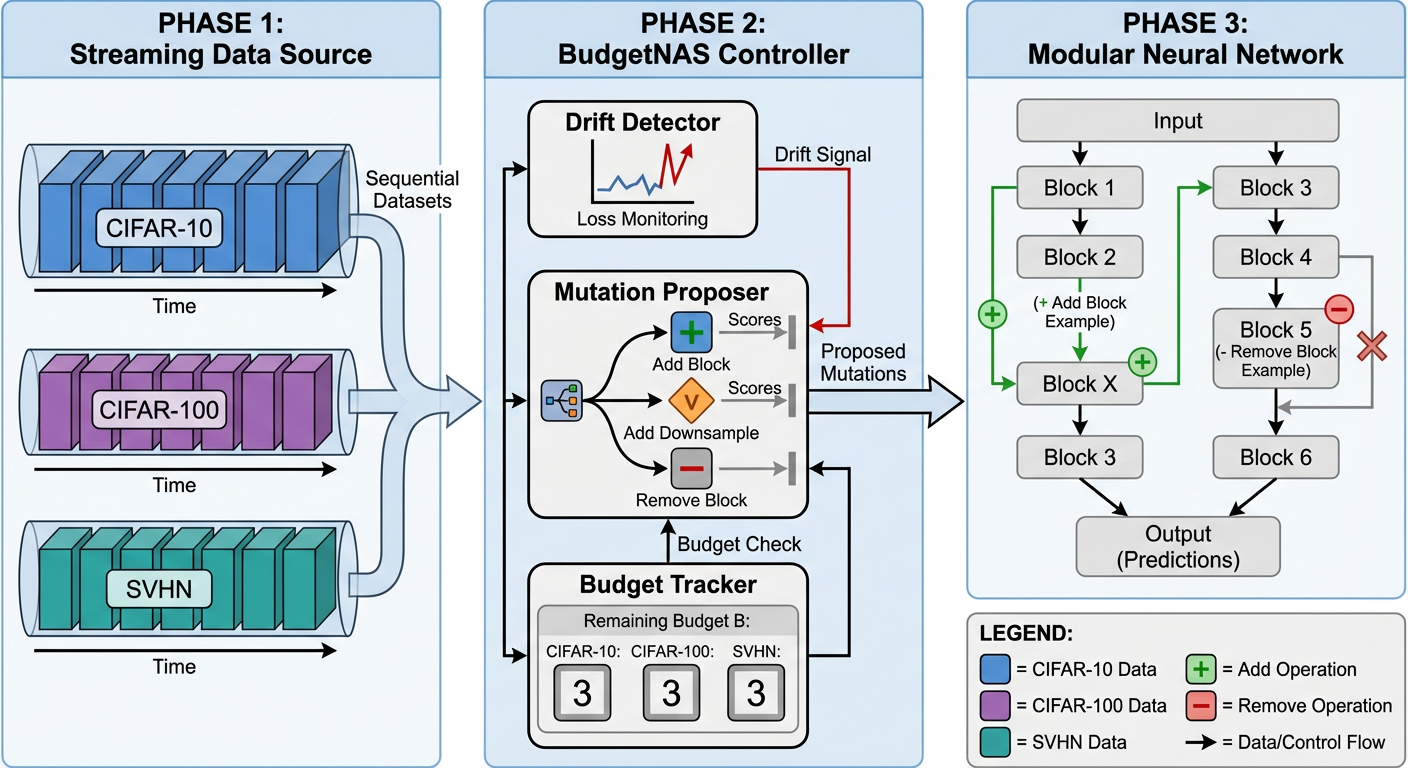
\includegraphics[width=\columnwidth]{fig_method_overview.png}
    \caption{\textbf{BudgetNAS Framework.} Data arrives in a task-incremental stream (left). The BudgetNAS Controller (center) monitors accuracy and proposes mutations under budget $B$. The modular network (right) is mutated selectively.}
    \label{fig:overview}
\end{figure}

\subsection{Modular Network Architecture}

We define a modular CNN composed of a fixed stem layer followed by mutable ResBlocks $\{b_1, \ldots, b_K\}$ and a task-specific classifier head. Each ResBlock contains two $3 \times 3$ convolutions with batch normalization, ReLU activations, and a skip connection. Three mutation operators modify the block sequence:

\begin{itemize}
    \item \textbf{AddBlock}: Appends a ResBlock with matching channel dimensions.
    \item \textbf{AddDownsample}: Appends a stride-2 ResBlock, doubling channels (up to 256), increasing the receptive field.
    \item \textbf{RemoveBlock}: Removes the second-to-last block (preserving the classifier interface).
\end{itemize}

When a new domain begins, the classifier head is replaced for the target classes. Existing feature extraction layers are preserved for transfer.

\subsection{BudgetNAS Controllers}

We investigate two controller designs:

\paragraph{Heuristic Controller.}
The controller maintains a per-domain budget~$B$ that resets at each domain transition. At the first chunk of each new domain (and any chunk where accuracy falls below threshold $\gamma = 0.35$), the controller proposes the highest-scoring feasible mutation:
\begin{equation}
    s(\text{mut}) = s_{\text{base}}(\text{mut}) + \beta \cdot \mathbb{1}[\text{acc} < \gamma]
\end{equation}
where $s_{\text{base}}$ assigns priors (AddBlock = 0.5, AddDownsample = 0.4, RemoveBlock = 0.2) and $\beta = 0.2$ is a low-accuracy bonus. The mutation is skipped if the budget is exhausted or accuracy exceeds~$\gamma$.

\paragraph{Bandit Controller.}
We also test a Thompson sampling~\cite{thompson1933likelihood,chapelle2011empirical} contextual bandit that maintains Beta($\alpha_a, \beta_a$) priors for each action $a \in \{\text{AddBlock, AddDownsample, RemoveBlock, NoOp}\}$. At each mutation opportunity, the controller samples from each action's posterior and selects the highest sample. After observing the outcome (accuracy change minus a parameter cost penalty: $r = \Delta\text{acc} - 0.05 \cdot \Delta\text{params}/10^6$), it updates the chosen action's Beta parameters.

\begin{algorithm}[t]
\caption{BudgetNAS Online Loop}
\label{alg:budgetnas}
\begin{algorithmic}[1]
\REQUIRE Stream $\mathcal{D}$, budget $B$, model $\mathcal{M}$, controller $C$
\FOR{each domain $d$ with known boundary}
    \STATE Replace classifier head for domain $d$
    \STATE Reset: $B_{\text{rem}} \leftarrow B$
    \FOR{each chunk $D_t$ in domain $d$}
        \STATE Train $\mathcal{M}$ on $D_t$ for $E$ epochs
        \STATE Evaluate: $\text{acc}_t$
        \IF{$B_{\text{rem}} > 0$ \AND $\text{acc}_t < \gamma$}
            \STATE $\text{mut}^* \leftarrow C.\text{propose}(\text{acc}_t, \mathcal{M})$
            \STATE Apply $\text{mut}^*$ to $\mathcal{M}$; $B_{\text{rem}} \leftarrow B_{\text{rem}} - 1$
        \ENDIF
    \ENDFOR
\ENDFOR
\end{algorithmic}
\end{algorithm}

\subsection{Stabilization Techniques (Ablated)}

We also evaluate two optional stabilization techniques, which we ultimately find to be \emph{counterproductive}:

\begin{itemize}
    \item \textbf{Warm-Start (WS)}: New blocks are initialized with Net2Net-style identity mappings~\cite{chen2016net2net} (second convolution weights set to zero so the residual path dominates initially).
    \item \textbf{Layer Freezing (FZ)}: After mutation, all blocks except the last two are frozen for one chunk, then unfrozen.
\end{itemize}

As shown in \Cref{sec:ablations}, both techniques reduce accuracy compared to random initialization, likely because identity-initialized blocks contribute too little during the critical first training chunk after mutation.

% ============================================================
% 4. EXPERIMENTS
% ============================================================
\section{Experiments}
\label{sec:experiments}

\subsection{Setup}

\paragraph{Streaming Benchmark.}
We construct a task-incremental streaming benchmark: CIFAR-10 (10 classes) $\rightarrow$ CIFAR-100 (100 classes) $\rightarrow$ SVHN (10 digit classes). Each dataset is split into 4 sequential chunks, yielding 12 streaming steps. We subsample 8K training and 2K test examples per dataset for computational tractability. All experiments use three random seeds (42, 123, 7) and we report mean $\pm$ std.

\paragraph{Methods Compared (10 total).}
We compare ten methods spanning four categories:

\emph{Fixed-architecture baselines:}
\textbf{(1)~Fixed}: 3-block ResNet retrained per domain.
\textbf{(2)~EWC}~\cite{kirkpatrick2017ewc}: Fixed architecture with elastic weight consolidation ($\lambda{=}400$).
\textbf{(3)~Exp.\ Replay}~\cite{chaudhry2019er}: Fixed architecture with 300-example replay buffer.

\emph{Unconditional growth:}
\textbf{(4)~Growing}: Adds 2 blocks at every domain transition.
\textbf{(5)~DEN-style}~\cite{yoon2018lifelong}: Adds 1 block per domain, freezes early blocks.
\textbf{(6)~Smart Growing}: Adds blocks only when accuracy $< 0.35$, with warm-start.

\emph{Random baseline:}
\textbf{(7)~RandomNAS} ($B{=}1$): Random mutation operator under the same budget.

\emph{BudgetNAS variants:}
\textbf{(8)~BudgetNAS-Heur} ($B{=}1$): Heuristic controller, no stabilization.
\textbf{(9)~BudgetNAS+WS+FZ} ($B{=}1$): Heuristic controller with warm-start and freezing.
\textbf{(10)~BudgetNAS-Bandit} ($B{=}1$): Thompson sampling controller.

\paragraph{Training.}
All models use SGD with momentum 0.9, weight decay $10^{-4}$, learning rate 0.02, and cosine annealing. Each chunk is trained for 3 epochs with batch size 256.

\subsection{Main Results}

\Cref{tab:results} reports final accuracy (mean $\pm$ std over 3 seeds) on each dataset, along with model size and the efficiency metric \emph{Gain/M} (mean accuracy divided by maximum parameter count in millions).

\begin{table*}[t]
\centering
\caption{\textbf{Final accuracy (\%, mean $\pm$ std, 3 seeds), model size, and efficiency.} Gain/M = mean final accuracy / max params (M). Best per column in \textbf{bold}, second-best \underline{underlined}. BudgetNAS-Heur achieves the best accuracy--efficiency tradeoff among architecture-changing methods.}
\label{tab:results}
\small
\begin{tabular}{@{}llccccccc@{}}
\toprule
& \textbf{Method} & \textbf{CIFAR-10} & \textbf{CIFAR-100} & \textbf{SVHN} & \textbf{Max Params} & \textbf{Blocks} & \textbf{Muts} & \textbf{Gain/M} \\
\midrule
\multirow{3}{*}{\rotatebox{90}{\scriptsize Fixed}}
& Fixed Backbone         & $41.7 \pm 0.8$ & $9.1 \pm 0.1$ & $28.2 \pm 1.0$ & 0.60M & 3 & 0 & 44.1 \\
& EWC                    & $41.7 \pm 0.8$ & $10.4 \pm 0.4$ & $26.6 \pm 0.3$ & 0.60M & 3 & 0 & 44.0 \\
& Exp.\ Replay           & $41.7 \pm 0.8$ & $8.6 \pm 0.3$ & $27.6 \pm 0.8$ & 0.60M & 3 & 0 & 43.5 \\
\midrule
\multirow{3}{*}{\rotatebox{90}{\scriptsize Growth}}
& Growing (Naive)        & $41.7 \pm 0.8$ & $\textbf{13.1} \pm 0.7$ & $\underline{37.7 \pm 3.6}$ & 1.77M & 7 & 4 & 17.5 \\
& DEN-style              & $41.7 \pm 0.8$ & $10.7 \pm 0.5$ & $28.4 \pm 1.0$ & 1.18M & 5 & 2 & 22.9 \\
& Smart Growing          & $39.0 \pm 4.1$ & $10.9 \pm 0.4$ & $31.1 \pm 1.1$ & 2.36M & 9 & 6 & 11.5 \\
\midrule
& RandomNAS ($B{=}1$)    & $38.5 \pm 4.0$ & $10.6 \pm 0.5$ & $32.7 \pm 7.5$ & 3.87M & 6 & 3 & 7.0 \\
\midrule
\multirow{3}{*}{\rotatebox{90}{\scriptsize Ours}}
& \textbf{BudgetNAS-Heur} ($B{=}1$)  & $\textbf{42.7} \pm 0.7$ & $\underline{11.6 \pm 0.5}$ & $35.6 \pm 1.3$ & 1.47M & 6 & 3 & \textbf{20.4} \\
& BudgetNAS+WS+FZ ($B{=}1$)          & $37.2 \pm 2.0$ & $8.9 \pm 0.2$ & $26.7 \pm 1.6$ & 1.47M & 6 & 3 & 16.5 \\
& BudgetNAS-Bandit ($B{=}1$)          & $36.3 \pm 1.3$ & $7.9 \pm 0.8$ & $\textbf{35.0} \pm 4.3$ & 2.98M & 6 & 3 & 8.9 \\
\bottomrule
\end{tabular}
\end{table*}

\begin{figure}[t]
    \centering
    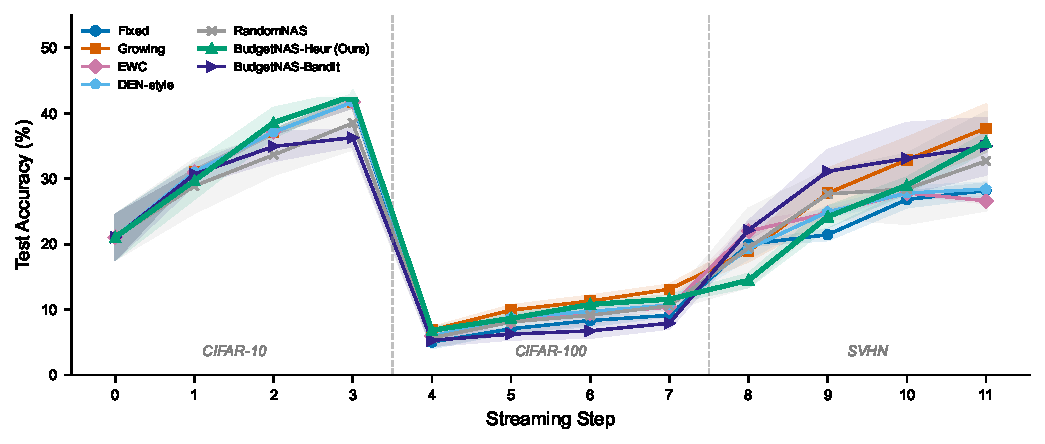
\includegraphics[width=\columnwidth]{fig2_accuracy_timeline.pdf}
    \caption{\textbf{Test accuracy over streaming steps} (mean $\pm$ std, 3 seeds, key methods shown). BudgetNAS-Heur (green, $\blacktriangle$) consistently tracks or exceeds baselines while using fewer parameters than Growing.}
    \label{fig:accuracy}
\end{figure}

\paragraph{Key Findings.}
(1)~\textbf{BudgetNAS-Heur is the best architecture-changing method by efficiency.} It achieves the highest CIFAR-10 accuracy ($42.7\%$, surpassing even fixed-architecture methods), second-highest CIFAR-100 ($11.6\%$), and strong SVHN ($35.6\%$) with only 1.47M parameters. Its Gain/M of 20.4 is the highest among all methods that modify architecture.
(2)~\textbf{Growing dominates on raw SVHN accuracy} ($37.7\%$) but at the cost of 1.77M parameters and zero selectivity.
(3)~\textbf{RandomNAS has extreme variance}: $7.5\%$ std on SVHN vs.\ $1.3\%$ for BudgetNAS-Heur---a $5.8\times$ variance reduction.
(4)~\textbf{Stabilization and bandit control both underperform} the simple heuristic (detailed in \Cref{sec:ablations}).

\begin{figure}[t]
    \centering
    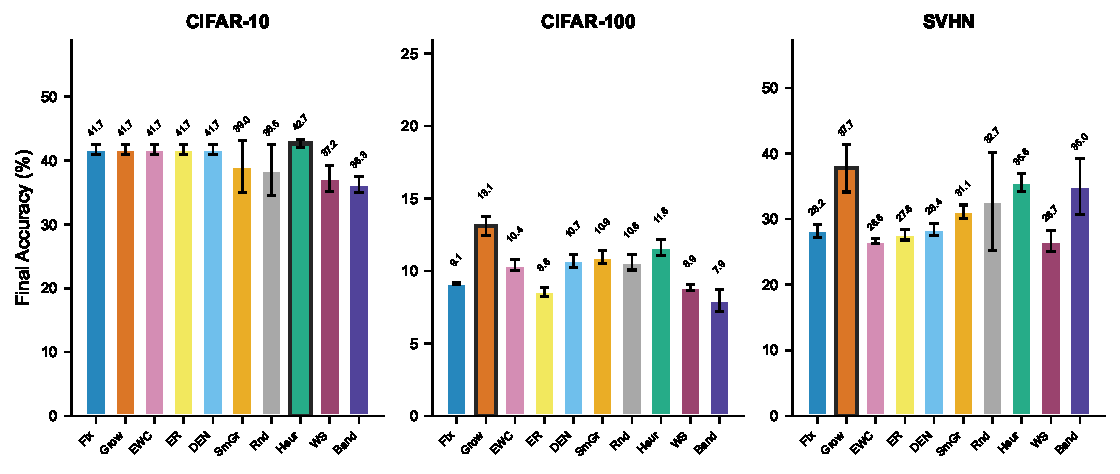
\includegraphics[width=\columnwidth]{fig3_final_comparison.pdf}
    \caption{\textbf{Final accuracy per dataset} (mean $\pm$ std, 3 seeds, all 10 methods). BudgetNAS-Heur (``Heur'') is competitive across all domains with low variance.}
    \label{fig:bars}
\end{figure}

\subsection{Ablation Studies}
\label{sec:ablations}

\paragraph{Budget Sweep ($B \in \{0,1,2,3,5\}$).}
We sweep the mutation budget using the bandit controller on seed~42 (\Cref{fig:budget}). $B{=}0$ (no mutations) yields a strong CIFAR-10 baseline ($41.9\%$) but poor SVHN ($24.2\%$). $B{=}1$ provides a large SVHN gain ($+6.4\%$). Beyond $B{=}2$, SVHN accuracy plateaus while CIFAR-10 degrades as early mutations disrupt the initial architecture. At $B{=}5$, SVHN accuracy \emph{drops back} to $24.6\%$---worse than $B{=}0$---demonstrating that excessive mutation is actively harmful. This confirms that $B{=}1$ is the practical sweet spot: enough capacity adaptation without optimization disruption.

\begin{figure}[t]
    \centering
    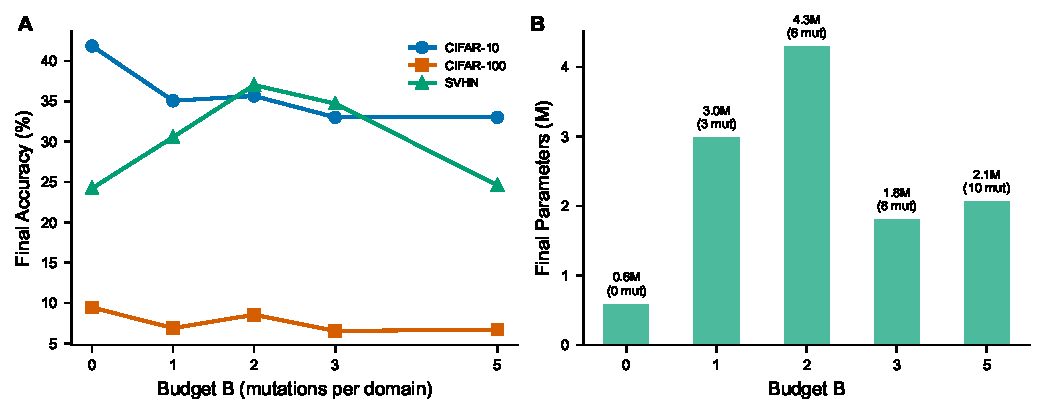
\includegraphics[width=\columnwidth]{fig4_budget_sweep.pdf}
    \caption{\textbf{Budget sweep.} \textbf{(A)} Final accuracy vs.\ budget $B$. $B{=}1$--$2$ provides the best tradeoff; $B{\geq}3$ degrades. \textbf{(B)} Parameter count grows with $B$.}
    \label{fig:budget}
\end{figure}

\paragraph{Trigger Ablation.}
We compare four mutation trigger conditions (seed~42, $B{=}1$, with warm-start): \emph{drift-only} (MMD-based drift detection), \emph{acc-only} (accuracy $< 0.35$), \emph{both}, and \emph{neither} (\Cref{fig:trigger}).

\begin{figure}[t]
    \centering
    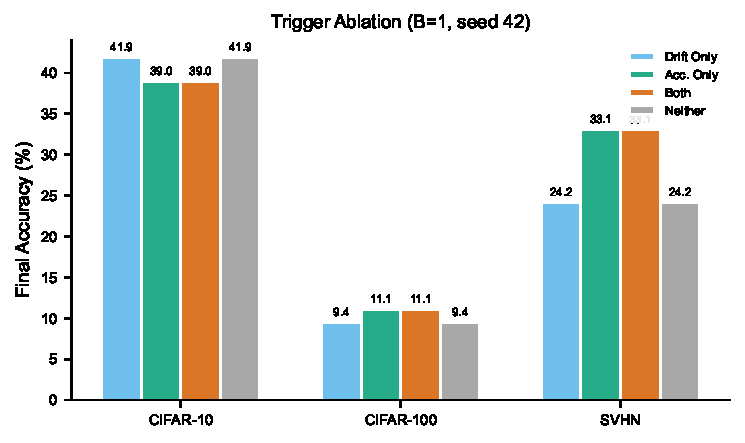
\includegraphics[width=\columnwidth]{fig5_trigger_ablation.pdf}
    \caption{\textbf{Trigger ablation.} Drift-only $=$ neither $=$ 0 mutations (drift never fires). Acc-only $=$ both $=$ 3 mutations. All benefit comes from the accuracy trigger.}
    \label{fig:trigger}
\end{figure}

The result is striking: \textbf{drift detection produces zero mutations}. The MMD-based detector never fires across the entire stream, making ``drift-only'' identical to ``neither'' (both yield 0~mutations and Fixed-equivalent accuracy). All mutations in the ``both'' condition come from the accuracy trigger, making it identical to ``acc-only.'' This finding simplifies the BudgetNAS controller: drift detection can be safely removed with no loss of functionality.

\paragraph{Stabilization Ablation.}
We compare four stabilization configurations (seed~42, $B{=}1$, heuristic controller): \emph{none} (random init), \emph{warm-start only}, \emph{freeze only}, and \emph{both} (\Cref{fig:stab}).

\begin{figure}[t]
    \centering
    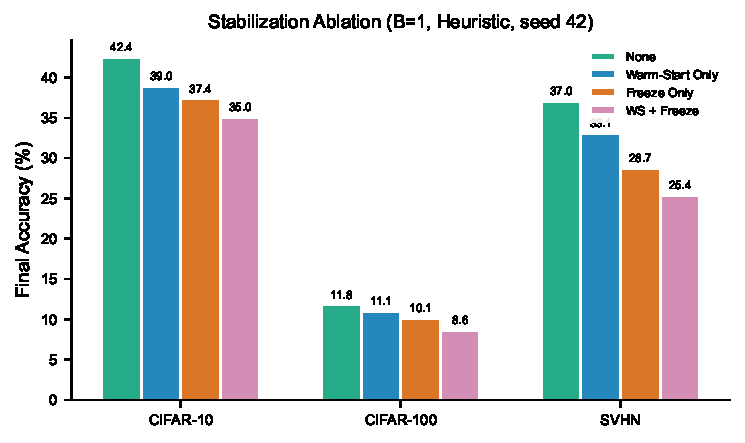
\includegraphics[width=\columnwidth]{fig6_stabilization_ablation.pdf}
    \caption{\textbf{Stabilization ablation.} Counterintuitively, no stabilization (``None'') outperforms all stabilization variants. Net2Net identity initialization makes new blocks too passive during the critical first training chunk.}
    \label{fig:stab}
\end{figure}

Counterintuitively, \textbf{no stabilization is best}: None ($42.4\%$, $11.8\%$, $37.0\%$) $>$ WS ($39.0\%$, $11.1\%$, $33.1\%$) $>$ FZ ($37.4\%$, $10.1\%$, $28.7\%$) $>$ WS+FZ ($35.0\%$, $8.6\%$, $25.4\%$). Each stabilization technique monotonically \emph{degrades} performance. We hypothesize that Net2Net identity initialization (zeroing the second convolution) makes new blocks too passive: they contribute minimally during the critical first training chunk, and the limited training budget (3 epochs per chunk) is insufficient for them to recover. Layer freezing compounds this by preventing early blocks from co-adapting with the new block. This is a \textbf{negative result} that contradicts the common assumption that function-preserving initialization helps in online settings with limited training.

\subsection{Gradual Shift}

We evaluate on a \emph{gradual shift} stream where blended transition chunks (50/50 mix) are inserted between domains (\Cref{fig:gradual}). BudgetNAS-Heur reaches $33.3\%$ on the final domain vs.\ $29.3\%$ for Fixed ($+4.0\%$ absolute). The bandit controller underperforms both ($24.9\%$), again confirming that the heuristic is more reliable at low budgets.

\begin{figure}[t]
    \centering
    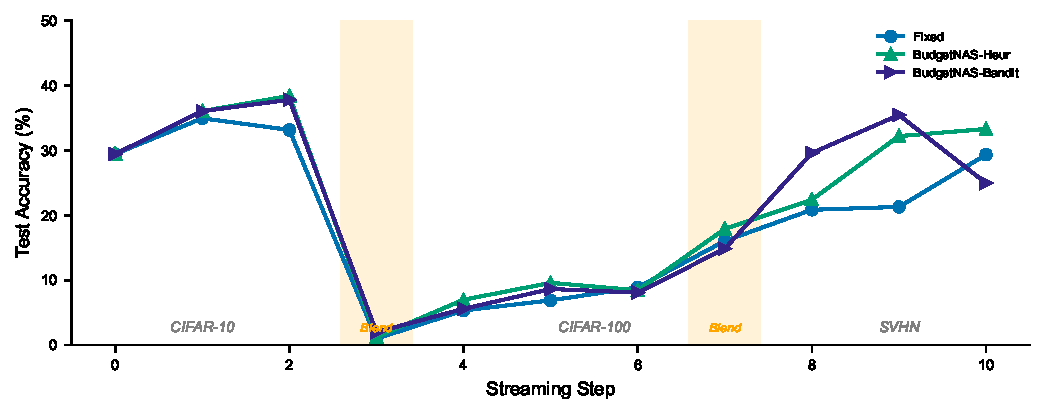
\includegraphics[width=\columnwidth]{fig7_gradual_shift.pdf}
    \caption{\textbf{Gradual shift stream.} Orange bands mark blended transition chunks. BudgetNAS-Heur outperforms Fixed by $+4.0\%$ on the final domain.}
    \label{fig:gradual}
\end{figure}

\subsection{Long Stream (4 Domains)}

We extend to a four-domain stream: CIFAR-10 $\rightarrow$ CIFAR-100 $\rightarrow$ SVHN $\rightarrow$ FashionMNIST (seed~42, \Cref{fig:long}). Growing achieves the highest FashionMNIST accuracy ($78.1\%$) by accumulating 7~blocks, while BudgetNAS-Bandit reaches $69.8\%$. RandomNAS achieves $79.9\%$ on FashionMNIST but with 3.87M parameters. This experiment reveals that BudgetNAS's conservative mutation strategy ($B{=}1$) may under-adapt on longer streams where more capacity is genuinely needed, suggesting that adaptive budget schedules deserve investigation.

\begin{figure}[t]
    \centering
    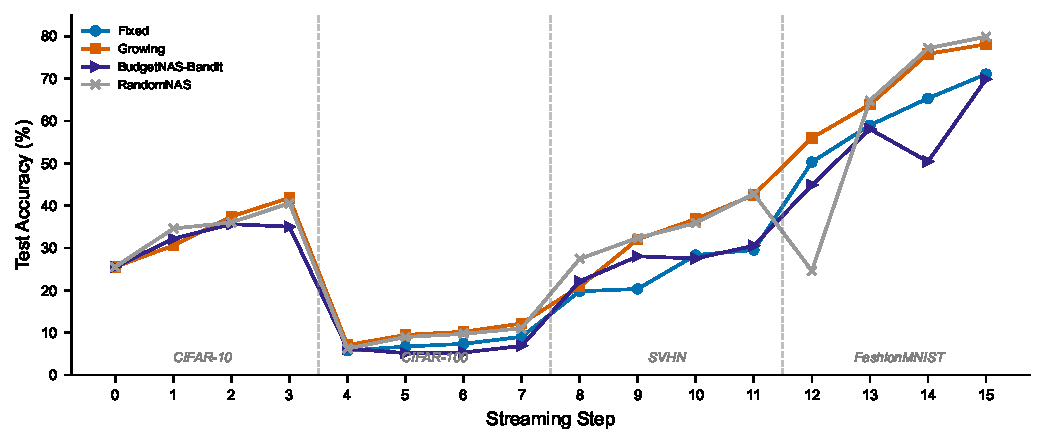
\includegraphics[width=\columnwidth]{fig8_long_stream.pdf}
    \caption{\textbf{Long stream (4 domains).} Growing and RandomNAS benefit from accumulated capacity on FashionMNIST; BudgetNAS-Bandit is competitive but constrained by $B{=}1$.}
    \label{fig:long}
\end{figure}

\subsection{Efficiency Analysis}

\Cref{fig:efficiency} visualizes the accuracy--efficiency tradeoff. Fixed-architecture methods cluster at high Gain/M (low params, moderate accuracy). Growing and Smart Growing trade efficiency for accuracy. BudgetNAS-Heur occupies the \emph{Pareto frontier}---higher accuracy than fixed methods at only $2.5\times$ the parameter cost, and comparable accuracy to Growing at $17\%$ fewer parameters.

\begin{figure}[t]
    \centering
    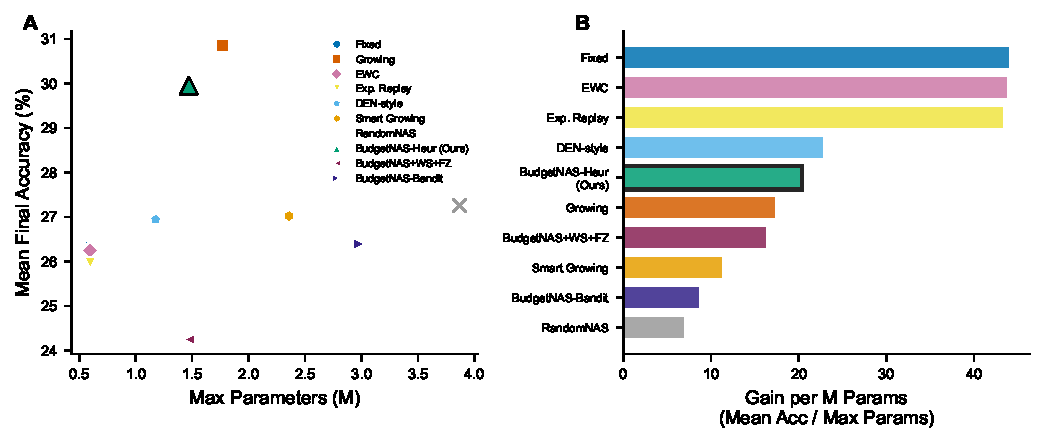
\includegraphics[width=\columnwidth]{fig9_efficiency.pdf}
    \caption{\textbf{Efficiency analysis.} \textbf{(A)} Accuracy vs.\ parameters scatter. \textbf{(B)} Gain/M ranking. BudgetNAS-Heur ($\blacktriangle$) achieves the best tradeoff among architecture-changing methods.}
    \label{fig:efficiency}
\end{figure}

% ============================================================
% 5. DISCUSSION
% ============================================================
\section{Discussion}
\label{sec:discussion}

\paragraph{Why the Heuristic Beats the Bandit.}
With $B{=}1$, the bandit controller observes only 3~mutation outcomes across the entire stream---far too few for Thompson sampling to learn meaningful action preferences. The heuristic's hard-coded bias toward AddBlock happens to be near-optimal for this benchmark, while the bandit wastes its limited budget on exploratory AddDownsample operations that increase parameters without proportional accuracy gains. At higher budgets ($B{\geq}3$), the bandit may have enough observations to learn, but higher budgets themselves degrade performance (see budget sweep). This creates a fundamental tension: the regime where budgeted mutation is most useful ($B{=}1$) is precisely where learned controllers have the least data.

\paragraph{Why Stabilization Hurts.}
The failure of warm-start contradicts Net2Net's success in offline transfer~\cite{chen2016net2net}. The key difference is training budget: Net2Net assumes extensive fine-tuning after morphism, while our streaming setting provides only 3 epochs per chunk. Identity-initialized blocks act as near-no-ops for the first chunk, effectively wasting $25\%$ of the domain's training on a block that barely contributes. Random initialization, while noisier, allows the new block to immediately participate in gradient flow.

\paragraph{Deployment Recommendation.}
Based on our experiments, we recommend the following configuration for practitioners deploying BudgetNAS:
\begin{enumerate}
    \item \textbf{Controller}: Heuristic with performance trigger ($\gamma = 0.35$).
    \item \textbf{Budget}: $B = 1$ per domain.
    \item \textbf{Initialization}: Random (not warm-start).
    \item \textbf{Freezing}: None.
    \item \textbf{Drift detection}: Not needed.
    \item \textbf{Preferred operator}: AddBlock (over AddDownsample).
\end{enumerate}

\paragraph{Limitations.}
(1)~The benchmark uses subsampled small-scale datasets; scaling to ImageNet remains open.
(2)~The heuristic's mutation priors are manually specified; sensitivity analysis across hyperparameter ranges would strengthen conclusions.
(3)~On the long stream, $B{=}1$ under-adapts for FashionMNIST, suggesting adaptive budgets may be needed for many-domain scenarios.
(4)~All methods share the same ResBlock architecture; heterogeneous blocks (e.g., attention, depthwise separable) could improve the mutation action space.
(5)~The task-incremental setting with known boundaries is simpler than class-incremental or boundary-free settings.

% ============================================================
% 6. CONCLUSION
% ============================================================
\section{Conclusion}
\label{sec:conclusion}

We introduced BudgetNAS, a framework for continual online NAS with explicit per-domain mutation budgets. Evaluating ten methods across three seeds with five ablation studies, we find that a simple heuristic controller with $B{=}1$ achieves the best accuracy--efficiency tradeoff: competitive accuracy with Growing at $17\%$ fewer parameters, $5.8\times$ lower variance than RandomNAS, and the highest Gain/M among architecture-changing methods. Our ablations reveal that several intuitively appealing design choices---drift detection, warm-start, layer freezing, learned controllers---are unnecessary or harmful at low mutation budgets. These negative results simplify the recommended BudgetNAS configuration to a single, easily-implemented rule: \emph{if accuracy is low, add one block}. We believe this simplicity is a strength: BudgetNAS requires no drift detectors, no function-preserving initialization, and no bandit learning---just performance monitoring and restrained architectural growth.

% ============================================================
% REFERENCES
% ============================================================
{
    \small
    \bibliographystyle{ieeenat_fullname}
    \bibliography{references}
}

\end{document}
